\documentclass[conference]{IEEEtran}
\IEEEoverridecommandlockouts

\usepackage{cite}
\usepackage{amsmath,amssymb,amsfonts}
\usepackage{algorithm}
\usepackage{algorithmic}
\usepackage{graphicx}
\usepackage{textcomp}
\usepackage{xcolor}
\usepackage{tikz}
\usepackage{booktabs}
\usepackage{listings}
\usepackage{hyperref}
\usetikzlibrary{arrows.meta, positioning, shapes.geometric}

\lstdefinestyle{py}{
  basicstyle=\ttfamily\scriptsize,
  keywordstyle=\color{blue!60!black},
  commentstyle=\color{gray},
  stringstyle=\color{purple!60!black},
  showstringspaces=false,
  breaklines=true,
  frame=single,
  numbers=none
}

\def\BibTeX{{\rm B\kern-.05em{\sc i\kern-.025em b}\kern-.08em
    T\kern-.1667em\lower.7ex\hbox{E}\kern-.125emX}}

\begin{document}

\title{Reach: A Governing Physical Agent Runtime for Delegating\\
Embodied Robot Tasks to Autonomous Computer-Use Systems}

\author{\IEEEauthorblockN{Anurag Dhiman}
\IEEEauthorblockA{Independent Researcher\\
anuragdhiman666@gmail.com}
}

\maketitle

\begin{abstract}
Many physical tasks that a robot performs have a digital sub-step: reading a value from a machine's
display and logging it, looking up a part number, filling in a report. Training every robot policy to also
drive a desktop or browser is wasteful and brittle. We present Reach, a system that instead composes
two independently-developed agents: a Physical Agent Runtime (PAR) that governs an embodied robot's
observation--plan--act loop, and a separate Autonomous Computer-Use System (ACS) that operates a
desktop computer. PAR exposes computer use to its own planner as a single, risk-tagged capability;
when the planner selects it, PAR's safety kernel decides whether the delegation may proceed unattended
or requires human approval, dispatches the task to the ACS over an explicit protocol, and folds the
result back into the robot's own action loop. We describe the capability/skill abstraction and two-stage
safety kernel that make this delegation auditable, a working reference implementation (Pulse as PAR,
CollectiveOS as the ACS) connected over a WebSocket bridge, and a physical-simulation integration that
reuses a ROS 2-shaped message schema without requiring ROS 2 itself. Beyond the single live delegation
reported previously, we now report a 31-experiment evaluation suite (of a pre-registered 33-experiment
plan) exercising core capability, safety-kernel behavior, delegation-decision quality, systems robustness,
and generality; a hardware-in-the-loop validation of the Webots bridge against a real installation,
closing a gap the original kinematic-fake validation left open; and a physically-real, non-anthropomorphic
manipulator that presses buttons on a small kiosk panel under contact confirmation from a touch sensor,
with the button choice made either by keyword matching or by a vision-language model reasoning over a
live camera image of the panel. We report what the evaluation suite found, including a real, disclosed
external-service outage that blocked one experiment's digital half, and discuss what remains before the
system has been exercised under real hardware or a standard agent benchmark.
\end{abstract}

\section{Introduction}
A robot that can see and manipulate its physical environment will, sooner or later, hit a step that is
not physical at all: it needs to read a machine's on-screen status, enter a measurement into a tracking
application, or submit a report before it can continue. One response is to train a single policy that jointly
grounds physical affordances and screen operation \cite{driess2023palme,brohan2023rt2}. We take a different, compositional approach: keep
the robot's governing runtime and a desktop-operating agent as two separate, independently maintained
systems, and make the decision to hand a task from one to the other an explicit, inspectable, safety-gated
event rather than an implicit property of a single learned policy.

This mirrors how large language model (LLM) agents already treat tools: a reasoning loop that decides,
at each step, whether to call an external capability and how to use its result before continuing \cite{yao2023react,schick2023toolformer}. Reach
generalizes this pattern one level up the stack -- the ``tool'' a physical robot calls is not a search API or a
calculator, but an entire autonomous agent that can perceive and operate a graphical desktop on the robot's
behalf.

Our contributions are:
\begin{itemize}
\item A capability/skill abstraction and a two-stage safety kernel (admission and policy checks with an
allow / modify / deny / escalate outcome) that governs when a robot's runtime may delegate a step
to an autonomous computer-use system, and requires human approval for that delegation under a
configurable risk profile.
\item A working reference bridge between an embodied runtime (Pulse, playing the role of PAR) and a screen-operating agent (CollectiveOS), connected over a minimal WebSocket protocol, with the delegation
recorded as an imitation-learning demonstration on the computer-use side.
\item A physical-simulation integration path (a Webots differential-drive robot), now validated against a
real Webots installation rather than only a hand-written kinematic fake, plus a physically-real,
non-anthropomorphic 2-axis gantry that presses buttons on a kiosk panel under touch-sensor
contact confirmation, with the button choice made by keyword matching or by a vision-language
model reading a live camera image.
\item A 31-experiment empirical evaluation (of a pre-registered 33-experiment plan spanning core
capability, safety, delegation intelligence, systems robustness, and generality/learning), reported
alongside the earlier single-run validation, with findings disclosed honestly including a real external
service outage that left one experiment's digital half inconclusive.
\end{itemize}

\section{Related Work}
\subsection{Embodied Language Agents}
\label{sec:embodied-agents}
SayCan \cite{ahn2022saycan} grounds an LLM's language-based planning in a learned affordance function so that proposed
actions are both plausible and physically feasible; Huang et al.\ \cite{huang2022zeroshot} show an LLM can propose actionable step
sequences for embodied tasks with only a translation step onto admissible actions. PaLM-E \cite{driess2023palme} and RT-2 \cite{brohan2023rt2}
go further and fold visual and physical grounding directly into a single multimodal model. Reach sits closer
to the first group: rather than fold computer-use competence into the robot's own model, it treats an entire
external agent as the thing being grounded and invoked.

\subsection{Tool Use and Reasoning in LLM Agents}
ReAct \cite{yao2023react} interleaves reasoning traces with actions so an LLM agent can call a tool, observe the result,
and revise its plan; Toolformer \cite{schick2023toolformer} shows a model can learn when to invoke a tool via self-supervision, and
Reflexion \cite{shinn2023reflexion} adds verbal self-critique after a failed attempt. Multi-agent frameworks such as AutoGen \cite{wu2023autogen}
and embodied, lifelong-learning agents such as Voyager \cite{wang2023voyager} treat other agents or skill libraries as callable
units much as we treat the autonomous computer-use system: a capability with a name, a description, and
a result that feeds back into the caller's own loop.

\subsection{Autonomous Computer-Use and GUI Agents}
WebArena \cite{zhou2024webarena} and Mind2Web \cite{deng2023mind2web} benchmark agents that must complete tasks by operating real web interfaces,
and CogAgent \cite{hong2024cogagent} targets GUI grounding directly from screenshots. Commercial computer-use agents that
perceive a screen and drive the mouse and keyboard, such as Anthropic's \cite{anthropic2024computeruse}, follow the same perceive--
plan--act--verify loop our ACS component implements. Reach does not propose a new computer-use agent;
it proposes a governed protocol for an \emph{external, physical} caller to invoke one.

\subsection{Robot Simulation Platforms}
Webots \cite{michel2004webots} and the Robot Operating System \cite{quigley2009ros} are the standard tooling for developing and testing robot
software before physical deployment; MuJoCo \cite{todorov2012mujoco} and Isaac Gym \cite{makoviychuk2021isaacgym} target high-throughput physics for
learning. Sim-to-real transfer typically relies on domain randomization \cite{tobin2017domain,peng2018simtoreal} to close the gap between
simulated and physical dynamics. Our simulation integration is narrower in scope: it does not attempt
sim-to-real transfer of a learned policy, only a faithful, physically-simulated stand-in for a mocked robot
interface, reusing a ROS 2-shaped schema so that a later move to ROS 2 itself is a transport change rather
than a redesign -- and, as of this evaluation, validated against a real Webots process rather than only a
kinematic fake (Section~\ref{sec:evaluation}).

\subsection{Safety-Governed Autonomy}
Amodei et al.\ \cite{amodei2016concrete} catalog concrete failure modes -- including unsafe exploration and reward hacking -- that
motivate building explicit safety layers around otherwise-capable agents rather than trusting a policy's own
judgment; Constitutional AI \cite{bai2022constitutional} pursues a complementary strategy of shaping the model's own behavior via
a set of stated principles. Reach's safety kernel is closer to the former: an external, non-learned gate that a
possibly-untrusted planner's proposed action must pass through, with an explicit human-escalation path for
high-risk capabilities.

\section{System Architecture}
\subsection{Overview}
Figure~\ref{fig:cycle} shows the delegation cycle. The robot perceives the physical world and proposes a next action
through its own planner; when that action is the \texttt{use\_computer} capability, PAR's safety kernel decides
whether to allow, modify, deny, or escalate it, dispatches an approved request to the ACS, and feeds the
ACS's result back into the robot's own observation--action loop so it can continue the physical task.

\begin{figure}[t]
\centering
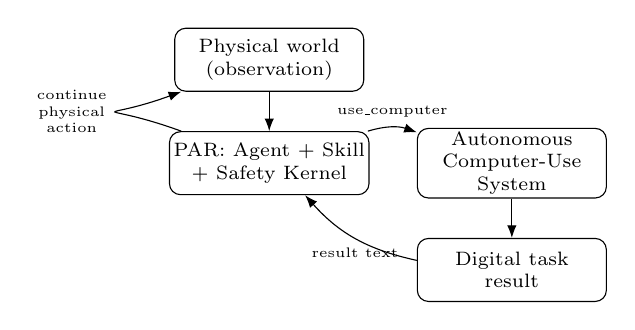
\begin{tikzpicture}[
  node distance=5mm and 6mm,
  box/.style={draw, rounded corners, align=center, minimum height=8mm, minimum width=24mm, font=\scriptsize, inner sep=1.5pt},
  lbl/.style={font=\tiny, align=center}
]
\node[box] (world) {Physical world\\(observation)};
\node[box, below=of world] (par) {PAR: Agent + Skill\\+ Safety Kernel};
\node[box, right=of par] (acs) {Autonomous\\Computer-Use\\System};
\node[box, below=of acs] (result) {Digital task\\result};

\draw[-{Latex[length=1.6mm]}] (world) -- (par);
\draw[-{Latex[length=1.6mm]}] (par) to[bend left=18] node[lbl, above]{use\_computer} (acs);
\draw[-{Latex[length=1.6mm]}] (acs) -- (result);
\draw[-{Latex[length=1.6mm]}] (result) to[bend left=18] node[lbl, below]{result text} (par);
\draw[-{Latex[length=1.6mm]}] (par) to[out=160,in=200,looseness=6] node[lbl, left]{continue\\physical\\action} (world);
\end{tikzpicture}
\caption{The Reach delegation cycle. PAR's planner proposes an action; a \texttt{use\_computer} action is safety-checked, dispatched to the ACS, and its result rejoins PAR's loop so the robot's physical task can continue.}
\label{fig:cycle}
\end{figure}

\subsection{Physical Agent Runtime (PAR)}
PAR implements a fixed loop -- Observation $\rightarrow$ Agent $\rightarrow$ Skill $\rightarrow$ Safety $\rightarrow$ Action -- around three data
types: an \texttt{Observation} (robot state and detected objects), an \texttt{Action} (a named skill with parameters),
and a \texttt{Capability} (a skill's declared name, description, input schema, risk level, and the environment
profiles it is valid under). A \texttt{Planner} maps a goal and the current observation to the next \texttt{Action}; we use
interchangeably a deterministic keyword-matching planner for testing and an LLM tool-use planner (Claude
or Gemini, following the ReAct pattern \cite{yao2023react}) for open-ended goals, both implementing the same interface so
the surrounding runtime is agnostic to which one is in use.

\subsection{Safety Kernel}
Every proposed action passes a two-stage check before it executes. The \emph{admission} stage rejects a capability outright if the runtime is in an emergency-stopped state or the capability is not registered for the
active environment profile. The \emph{policy} stage evaluates the specific action against that profile's constraints
(workspace bounds, collision margin against currently-detected objects, velocity limits) and returns one of
four outcomes: \textsc{Allow}, \textsc{Modify} (e.g.\ a move target is speed-clamped to a reachable distance), \textsc{Deny}, or
\textsc{Escalate} to a human-approval callback. A denial is fed back to the planner rather than aborting the task,
so the agent re-plans around it -- Algorithm~\ref{alg:safety} summarizes the check for the capability at the center of this
paper.

We mark \texttt{use\_computer} as \textsc{High} risk. Combined with a profile that requires approval, this forces a
human-approval escalation before any delegation to the ACS in a real-robot deployment; under a permissive
simulation profile it runs unattended, which is what let us validate the loop without a human in it for every
step.

\begin{algorithm}[t]
\caption{Safety check for a proposed action}
\label{alg:safety}
\begin{algorithmic}[1]
\REQUIRE action $a$, observation $o$, capability $c$, profile $p$
\IF{emergency stop engaged}
  \RETURN \textsc{Deny}
\ENDIF
\IF{$p.\text{name} \notin c.\text{env\_profiles}$}
  \RETURN \textsc{Deny} \COMMENT{admission stage}
\ENDIF
\IF{$c.\text{risk} = \textsc{High}$ \AND $p.\text{approval\_required}$}
  \RETURN \textsc{Escalate}
\ENDIF
\IF{$a.\text{skill} = \texttt{move}$}
  \RETURN CheckMove$(a, o, p)$ \COMMENT{workspace / collision / velocity}
\ENDIF
\RETURN \textsc{Allow}
\end{algorithmic}
\end{algorithm}

\begin{table}[t]
\centering
\caption{Wire protocol between PAR and the ACS (JSON over WebSocket)}
\label{tab:wire}
\begin{tabular}{@{}ll@{}}
\toprule
Robot $\rightarrow$ ACS & ACS $\rightarrow$ Robot \\
\midrule
\{"type":"task", & \{"type":"reply", \\
\ "text":\textless{}task\textgreater{}\} & \ "text":\textless{}result\textgreater{}, \\
 & \ "status":\textless{}done\textbar{}error\textgreater{}\} \\
\bottomrule
\end{tabular}
\end{table}

\subsection{Autonomous Computer-Use System (ACS)}
\label{sec:acs}
The ACS (CollectiveOS in our implementation) runs a perceive--plan--act--verify loop over a real desktop: it
captures a screenshot and the platform accessibility tree, plans a short sequence of sub-steps with a vision-language model, grounds and executes each step through UI automation or browser control, and verifies
the action changed the screen as expected before continuing -- the same shape of loop used by GUI-agent
benchmarks and systems \cite{zhou2024webarena,deng2023mind2web,hong2024cogagent,anthropic2024computeruse}. Write-flavored actions (send, delete, purchase, \ldots) are meant to pause
for human-in-the-loop confirmation when the ACS is driven through its own chat interface; critically, that
confirmation gate is not wired into the robot-facing endpoint described next, which is why PAR's own safety
kernel is load-bearing for this integration rather than a convenience.

\subsection{The Bridge}
PAR exposes computer use to its planner as a single capability, \texttt{use\_computer}, taking one parameter (\texttt{task},
a natural-language description of the digital step). When the planner selects it and the safety kernel allows
or approves it, a robot-interface wrapper forwards the request over a WebSocket connection to the ACS's
robot-facing endpoint, which runs its computer-use loop synchronously and replies with a status and a
natural-language result (Table~\ref{tab:wire}). The reply is translated back into PAR's own \texttt{ActionResult} type, so from
the rest of PAR's perspective a delegated computer step looks exactly like any other skill's result -- success or
failure, with a message the planner can read and react to. Every such run is also recorded by the ACS as an
imitation-learning demonstration (a before-screenshot paired with the action taken at each step), which is
the data trail this delegation protocol produces toward a robot eventually \emph{learning} to use a computer rather
than only delegating it.

A network failure, a timeout, or an authentication error is caught at the bridge and returned as a normal
failed result rather than an exception, so a delegation that cannot reach the ACS is something the planner
can observe and re-plan around, in keeping with the safety kernel's own denial-is-recoverable design. Our
evaluation suite exercises this path directly with an external failure that was not staged (Section~\ref{sec:e18}).

\begin{table}[t]
\centering
\caption{Implementation stack}
\label{tab:stack}
\begin{tabular}{@{}ll@{}}
\toprule
Concern & Choice \\
\midrule
Language & Python \\
Data validation & Pydantic \\
PAR planners & Rule-based; Claude / Gemini tool-use \\
ACS API layer & FastAPI, WebSocket \\
ACS task loop & LangGraph \\
ACS screen control & Accessibility tree, browser automation, \\
 & pointer/keyboard automation \\
PAR $\leftrightarrow$ ACS transport & WebSocket, JSON payloads \\
Physical simulation & Webots \\
\bottomrule
\end{tabular}
\end{table}

\subsection{Physical Simulation Integration}
\label{sec:webots-integration}
To evaluate whether the safety kernel's physical checks (workspace bounds, collision margin) behave sensibly
against something more than an in-memory mock, we bridged PAR to a physically-simulated differential-drive
robot in Webots \cite{michel2004webots}. PAR already supports a ROS 2 robot interface with a pure, transport-agnostic JSON
mapping between its \texttt{Observation}/\texttt{Action} types and a wire payload; because our development environment
had no official ROS 2 build for its OS/CPU combination and very little free disk for a full ROS 2 or
virtual-machine install, we reused that same JSON mapping over a plain WebSocket to an external Webots
controller process instead of ROS 2 topics. The bridge controller runs a point-and-shoot controller for the
\texttt{move} capability -- rotate in place to face the target within a heading tolerance, drive straight while re-checking
heading, stop within a distance tolerance -- and answers \texttt{detect}/\texttt{inspect} via direct supervisor queries of
known objects' world positions, which are the same positions the safety kernel's collision check consumes, so
a collision denial exercises identically whether the robot behind PAR is the in-memory mock or the simulated
one. Section~\ref{sec:evaluation} reports this bridge validated against a real Webots installation, not only the kinematic
fake it was first checked against.

\subsection{Physically-Real Computer-Use Delegation}
\label{sec:gantry}
The integration above lets a wheeled robot navigate and have its physical safety checks exercised for real, but
the robot itself has no way to type or click -- a delegated \texttt{use\_computer} step still operates the real host
desktop through the ACS, with the robot only \emph{symbolically} docking at a laptop prop in the simulated arena
(driving to a fixed offset from it and lighting an indicator LED for the delegation's duration) so the hand-off
is visible in the simulation rather than happening invisibly off to the side.

To make at least a bounded class of computer-use delegations \emph{physically} real rather than symbolic, we added
a second simulated robot to the arena: a fixed, non-anthropomorphic 2-axis (X+Z) gantry mounted over a
small kiosk panel of three buttons. A \texttt{SliderJoint}-driven linear motor on each axis moves a plunger tip to
one of three X positions and presses downward; contact is confirmed by a touch sensor on the plunger tip,
polled continuously during the press rather than only after the motor reports it has arrived, since the
contact force proved to be a brief transient rather than a sustained value. The panel runs a small, genuinely
stateful scripted application on an attached display (idle $\rightarrow$ an alert shown after \texttt{check} $\rightarrow$
\texttt{confirm}/\texttt{clear} return it to idle), so a press has a real, observable digital effect, not a decorative one.

Two interchangeable decision strategies choose which button to press for a given \texttt{use\_computer} task,
selected by an environment variable so neither the capability's interface nor the rest of the delegation path
needs to change: a keyword-matching bridge maps a small fixed vocabulary in the task text to a button; and a
vision-guided bridge instead captures a live image from a camera mounted beside the gantry's carriage,
sends it together with the task text to a vision-language model (Gemini, \texttt{gemini-3.1-flash-lite}) constrained to a
three-way structured response, and presses whichever button the model names, failing cleanly if it names
none. We verified the vision-guided path end to end against the kiosk's genuine starting state (idle,
\emph{not} staged): the model's own stated reasoning was that the panel was idle and so the \texttt{check} button -- not
\texttt{confirm} -- should be pressed, and the gantry then pressed it for real, changing the panel's displayed state.
This is a narrower, decision-grounded instance of the same perceive-then-act pattern the ACS itself
implements against a real desktop (Section~\ref{sec:acs}), applied here to a three-way physical choice rather than
general screen operation.

This is a deliberately modest step toward the dexterous-manipulation, learned-policy vision that motivates
much of the embodied-agent literature we build on (Section~\ref{sec:embodied-agents}): a fixed gantry pressing one of three large
buttons is not a general-purpose manipulator, it does not grasp or manipulate a real keyboard and mouse,
and its vision-guided decision is a closed three-way classification, not open-ended GUI grounding. We
report it as a concrete, physically-verified instance of a non-anthropomorphic manipulator carrying out a
real digital interaction under sensor-confirmed contact, and as a bounded testbed for grounding a
delegation decision in a live image rather than text alone -- not as a solution to general robotic computer use.

\section{Implementation}
PAR (Pulse) and the ACS (CollectiveOS) are independent Python code bases communicating only over
the protocols described above; each also embeds its own LLM client (Claude or Gemini for PAR's planner,
Gemini for the ACS's perception/planning) behind an interface so either can be swapped. The ACS's own
conversational surface is a FastAPI service with a LangGraph-based task loop; PAR is a plain library with
no server component of its own -- it is a runtime a robot's control process links against directly. Table~\ref{tab:stack}
summarizes the stack.

\section{Evaluation}
\label{sec:evaluation}
We report what has and has not been exercised, in two parts: the single live delegation and kinematic-fake
bridge validation reported previously, and a 31-experiment empirical evaluation suite completed since, drawn
from a pre-registered 33-experiment plan spanning five categories. Two experiments in that plan remain
genuinely blocked -- both require a real human operator making timed approval decisions, which we could
not substitute for -- and are reported as such rather than silently omitted.

\subsection{Live Delegation and Bridge Validation (Prior Result)}
We ran a read-only task end to end: PAR's runtime, under the safety kernel's escalation gate, delegated
``which application is currently in the foreground?'' to a live instance of the ACS. The ACS's vision-language
model correctly identified the foreground application, and the result returned through PAR's normal
\texttt{ActionResult} path. A transient upstream rate-limit error on a first attempt surfaced as an ordinary failed
result rather than a crash, and a retry succeeded. PAR's and the ACS's unit and integration test suites,
including regression tests added after finding and fixing an authentication bug that had made the ACS's
robot-facing WebSocket endpoint entirely unreachable, pass in full.

\subsection{Hardware-in-the-Loop Webots Validation (New)}
\label{sec:webots-real}
The Webots bridge (Section~\ref{sec:webots-integration}) was previously validated only against a hand-written kinematic fake, with the
real Webots API surface -- device and node names, coordinate-system handling -- explicitly left unverified.
We subsequently obtained a working Webots R2025a installation and ran two experiments directly against it.
The first re-evaluated the same safety-kernel scenario battery used for the in-memory ablation study
(Section~\ref{sec:ablation}) against a live Webots robot's observation alongside the in-memory mock's, in the same run: both
reached perfect decision accuracy on all ten scenarios and agreed with each other on every one, indicating
the kernel's decision depends only on the observation's values, not on which concrete robot interface
produced it. The second drove one real sequence through the full pipeline -- waypoint navigation and target
approach (converging within a 5\,cm tolerance), a live collision-margin denial against a real detected
object's position, a live workspace-bound denial, and emergency-stop (blocking the next action, then
recovering once cleared) -- all against the live simulator; every check passed, closing the gap the original
kinematic-fake validation left open.

\begin{table}[t]
\centering
\caption{Evaluation suite summary, by category (31 of 33 attempted)}
\label{tab:suite}
\small
\begin{tabular}{@{}p{0.15\linewidth}p{0.10\linewidth}p{0.65\linewidth}@{}}
\toprule
Category & $N$ & Headline finding \\
\midrule
Core Capability & 4 & Live delegation succeeds but is unreliable end to end (12-trial pilot: most non-completions traced to quota limits, a real intermittent screenshot-capture race, or expected \texttt{max\_iter} outcomes -- zero unexplained failures). \\
Safety & 4 + 1 bl. & Full safety kernel reaches 0\% unsafe-execution rate and perfect four-outcome decision accuracy on the scenario battery; e-stop reliably blocks actions and the ACS is never contacted while engaged; escalation is driven by a capability's fixed risk tag, not the content of a given task. \\
Delegation Intelligence & 5 & An LLM planner's decision \emph{to} delegate scored perfect precision/recall on a small scored set; but planner choice is pivotal -- a rule-based planner reached 0\% task success on natural-language goals where an LLM planner reached 69\%. \\
Systems Robustness & 9 + 1 bl. & The bridge degrades safely under fault injection and scales cleanly to 8 concurrent robot clients; but two real design gaps surfaced: PAR accepts an incorrect or ambiguous ACS result as success identically to a correct one (no semantic verification exists), and an all-denials task can exhaust its step budget stuck in \texttt{PLANNING}, reaching neither \texttt{DONE} nor \texttt{FAILED}. \\
Generality \& Learning & 4 & 44 real delegation attempts yielded 14 recorded demonstrations; a toy nearest-neighbor model over them correctly predicted a held-out task's action type, a small proof of concept toward imitation learning from delegated runs, not a trained policy. \\
\bottomrule
\end{tabular}
\end{table}

\subsection{Evaluation Suite (New)}
\label{sec:ablation}
Table~\ref{tab:suite} summarizes the suite by category; full per-experiment design, metrics, and raw trial records are
reported in the project repository rather than reproduced in full here, in the interest of space. We highlight
three findings we consider load-bearing for how the architecture should be read. First, the safety kernel's
contribution is real and separable: an admission-only configuration (emergency-stop and profile checks, no
policy-stage checks) still blocks the scenarios that are admission-stage violations but allows every
workspace, collision, and risk-escalation violation through, confirming the two-stage design is not
redundant with itself. Second, delegation \emph{decision} quality and delegation \emph{execution} quality are
different questions with different answers: the LLM planner we evaluated chose to delegate exactly when it
should on every scored trial, but whether the delegated task then actually completed depended heavily on
external service availability (Section~\ref{sec:e18}) and on real, intermittent bugs in the ACS's own perception step --
neither of which the delegation decision itself controls. Third, the evaluation surfaced two genuine
correctness gaps that unit testing had not: PAR has no mechanism to verify an ACS result's content before
treating it as a successful completion, and a task that is denied at every step can become permanently
stuck rather than terminating in a reportable failure state. Both are concrete, scoped items for future work
(Section~\ref{sec:future}) rather than properties we consider acceptable as shipped.

\subsection{A Disclosed External Outage (E18)}
\label{sec:e18}
One experiment specifically composes the physical and digital halves in a single task: a simulated robot
navigates, is denied a collision, navigates again, and then delegates a real digital sub-task to a live ACS
instance before the task can complete. We attempted this three times against a live Webots process and a
live CollectiveOS instance. In all three attempts the physical half succeeded identically -- the same
waypoint navigation and live collision denial reported in Section~\ref{sec:webots-real}, now exercised as part of a composed
task rather than in isolation. In all three attempts the digital half failed with an identical ``high demand''
(HTTP 503) error from the underlying vision-language API, across both of the two Gemini models available
to us, one of which carries a hard daily request cap we were unwilling to spend further probing an outage
we judged, after three identical failures, to be a genuine service-side degradation rather than noise. The
runtime's own documented contract -- a genuine execution failure, unlike a safety denial, ends a task's
step loop rather than continuing past it -- behaved exactly as designed in all three attempts: the failure
surfaced as an ordinary failed result with a readable message, not a crash, and the scripted remainder of
the task was correctly never reached. We report this experiment as attempted and informative rather than
blocked: it independently reconfirms, from a different angle, a same-day finding from a separate
generalization experiment that also hit a sustained outage on the same model, and it is the clearest
evidence in this evaluation that the bridge's failure handling (Section~\ref{sec:webots-integration}) behaves as designed under a real,
unstaged external failure -- we simply did not obtain a fully successful composed run before judging further
attempts an unproductive use of scarce quota.

\section{Discussion and Limitations}
The current ROS 2 robot interface executes fire-and-forget, with no completion acknowledgement from the
physical robot -- a limitation we inherited rather than fixed, since our simulation work deliberately avoided
that interface. A real deployment migrating from the WebSocket bridge to ROS 2 (on hardware where ROS 2
is available) should close that gap rather than carry it forward.

The evaluation suite resolved two of the three open questions the original preliminary evaluation posed, and
sharpened the third. Whether an LLM planner reliably chooses to delegate only when a step genuinely needs
a computer now has a preliminary, positive answer on a small scored set (Section~\ref{sec:ablation}); whether the Webots
bridge's real API surface matches its kinematic-fake validation now has a positive answer as well
(Section~\ref{sec:webots-real}). What the suite instead sharpened is end-to-end reliability: a live delegation can be denied
completion by causes entirely outside the delegation decision itself -- a daily or per-minute quota limit, an
intermittent screenshot-capture race in the ACS, or, as in Section~\ref{sec:e18}, a sustained upstream outage -- so a
single success-rate number conflates architectural correctness with the current reliability of third-party
services we do not control, and should be read with that caveat rather than at face value.

The evaluation also surfaced two correctness gaps worth stating plainly rather than minimizing. PAR
currently performs no semantic verification of a returned ACS result before treating it as success, which
means an incorrect or ambiguous digital answer is indistinguishable, from PAR's side, from a correct one.
And a task that is denied at every proposed step can exhaust its step budget without ever reaching a
terminal \texttt{DONE} or \texttt{FAILED} state, which is a real gap in how the runtime reports an unrecoverable
situation rather than a cosmetic one. Neither undermines the safety kernel's own denial behavior, which
remains correct in isolation; both are about what the runtime does with a stream of denials or unverifiable
results over a longer task.

Finally, the current authentication between PAR and the ACS remains a single shared secret; a dedicated
evaluation of this boundary confirmed it is adequate for one robot and one ACS instance in development but
not for a multi-robot or multi-tenant deployment, and that a valid token can be replayed -- a known,
disclosed limitation rather than a newly discovered one, now with a concrete evaluation behind the claim.

\section{Future Work}
\label{sec:future}
Immediate priorities are: (1) re-attempting the composed physical+digital task (Section~\ref{sec:e18}) once the
underlying vision-language API's availability has recovered, to obtain a fully successful real run rather than
three physically-successful-but-digitally-blocked ones; (2) closing the two correctness gaps the evaluation
suite surfaced -- result-content verification for ACS responses, and a terminal failure state for an
all-denials task -- both scoped and reproducible rather than speculative; (3) extending the physically-real
gantry (Section~\ref{sec:gantry}) toward genuine grasping manipulation of a real keyboard and mouse, and toward a
vision-guided decision over open-ended screen content rather than a closed three-way button choice, which
remains the larger and harder version of the dexterous-manipulation vision this work only takes a first,
deliberately modest step toward; (4) growing the imitation-learning proof of concept (Section~\ref{sec:ablation}) from a toy
nearest-neighbor baseline over 14 demonstrations into an actually-trained policy over a substantially larger
demonstration set; and (5) adapting a GUI-agent benchmark such as WebArena \cite{zhou2024webarena} or Mind2Web \cite{deng2023mind2web}
to be invoked through a robot planner, rather than directly, which remains the clearest path to a
standardized comparison this evaluation does not yet provide.

\section{Conclusion}
Reach shows that a robot's need to occasionally use a computer does not require folding computer-use
competence into the robot's own policy. A small, explicit capability, gated by a two-stage safety kernel
with a human-escalation path, is enough to compose a physical agent runtime with an independently-built autonomous computer-use system, and the same schema-preserving approach extends to a physically-simulated robot without requiring a full ROS 2 toolchain. Beyond the single live task reported previously, a
31-experiment evaluation suite and a hardware-in-the-loop Webots validation move this from a preliminary
systems check toward a broader empirical account of where the architecture holds up and where it does
not -- including two genuine correctness gaps and a real external-service outage, reported here rather than
smoothed over. A physically-real, non-anthropomorphic gantry extends the delegation path beyond a
symbolic docking gesture into a sensor-confirmed physical action, with the choice of action grounded in a
live camera image rather than text alone. The honest next step is still broader, harder validation: on real
hardware, against a standardized benchmark, and with the two surfaced correctness gaps closed rather than
only documented.

\section*{Acknowledgments}
This system and this paper were developed with the assistance of Claude (Anthropic).

\begin{thebibliography}{21}

\bibitem{ahn2022saycan}
M.~Ahn \emph{et al.}, ``Do As I Can, Not As I Say: Grounding Language in Robotic Affordances,'' \emph{arXiv preprint arXiv:2204.01691}, 2022.

\bibitem{huang2022zeroshot}
W.~Huang, P.~Abbeel, D.~Pathak, and I.~Mordatch, ``Language Models as Zero-Shot Planners: Extracting Actionable Knowledge for Embodied Agents,'' in \emph{Proc. ICML}, 2022, arXiv:2201.07207.

\bibitem{driess2023palme}
D.~Driess \emph{et al.}, ``PaLM-E: An Embodied Multimodal Language Model,'' in \emph{Proc. ICML}, 2023, arXiv:2303.03378.

\bibitem{brohan2023rt2}
A.~Brohan \emph{et al.}, ``RT-2: Vision-Language-Action Models Transfer Web Knowledge to Robotic Control,'' \emph{arXiv preprint arXiv:2307.15818}, 2023.

\bibitem{yao2023react}
S.~Yao \emph{et al.}, ``ReAct: Synergizing Reasoning and Acting in Language Models,'' in \emph{Proc. ICLR}, 2023, arXiv:2210.03629.

\bibitem{schick2023toolformer}
T.~Schick \emph{et al.}, ``Toolformer: Language Models Can Teach Themselves to Use Tools,'' in \emph{Proc. NeurIPS}, 2023, arXiv:2302.04761.

\bibitem{shinn2023reflexion}
N.~Shinn, F.~Cassano, A.~Gopinath, K.~Narasimhan, and S.~Yao, ``Reflexion: Language Agents with Verbal Reinforcement Learning,'' in \emph{Proc. NeurIPS}, 2023, arXiv:2303.11366.

\bibitem{zhou2024webarena}
S.~Zhou \emph{et al.}, ``WebArena: A Realistic Web Environment for Building Autonomous Agents,'' in \emph{Proc. ICLR}, 2024, arXiv:2307.13854.

\bibitem{deng2023mind2web}
X.~Deng \emph{et al.}, ``Mind2Web: Towards a Generalist Agent for the Web,'' in \emph{Proc. NeurIPS}, 2023, arXiv:2306.06070.

\bibitem{hong2024cogagent}
W.~Hong \emph{et al.}, ``CogAgent: A Visual Language Model for GUI Agents,'' in \emph{Proc. CVPR}, 2024, arXiv:2312.08914.

\bibitem{wu2023autogen}
Q.~Wu \emph{et al.}, ``AutoGen: Enabling Next-Gen LLM Applications via Multi-Agent Conversation,'' \emph{arXiv preprint arXiv:2308.08155}, 2023.

\bibitem{wang2023voyager}
G.~Wang \emph{et al.}, ``Voyager: An Open-Ended Embodied Agent with Large Language Models,'' \emph{arXiv preprint arXiv:2305.16291}, 2023.

\bibitem{michel2004webots}
O.~Michel, ``Cyberbotics Ltd. Webots\texttrademark: Professional Mobile Robot Simulation,'' \emph{International Journal of Advanced Robotic Systems}, vol.~1, no.~1, pp.~39--42, 2004.

\bibitem{quigley2009ros}
M.~Quigley \emph{et al.}, ``ROS: an open-source Robot Operating System,'' in \emph{ICRA Workshop on Open Source Software}, 2009.

\bibitem{todorov2012mujoco}
E.~Todorov, T.~Erez, and Y.~Tassa, ``MuJoCo: A physics engine for model-based control,'' in \emph{Proc. IEEE/RSJ IROS}, 2012, pp.~5026--5033.

\bibitem{makoviychuk2021isaacgym}
V.~Makoviychuk \emph{et al.}, ``Isaac Gym: High Performance GPU-Based Physics Simulation For Robot Learning,'' \emph{arXiv preprint arXiv:2108.10470}, 2021.

\bibitem{amodei2016concrete}
D.~Amodei, C.~Olah, J.~Steinhardt, P.~Christiano, J.~Schulman, and D.~Man\'e, ``Concrete Problems in AI Safety,'' \emph{arXiv preprint arXiv:1606.06565}, 2016.

\bibitem{bai2022constitutional}
Y.~Bai \emph{et al.}, ``Constitutional AI: Harmlessness from AI Feedback,'' \emph{arXiv preprint arXiv:2212.08073}, 2022.

\bibitem{tobin2017domain}
J.~Tobin \emph{et al.}, ``Domain Randomization for Transferring Deep Neural Networks from Simulation to the Real World,'' in \emph{Proc. IEEE/RSJ IROS}, 2017, arXiv:1703.06907.

\bibitem{peng2018simtoreal}
X.~B.~Peng, M.~Andrychowicz, W.~Zaremba, and P.~Abbeel, ``Sim-to-Real Transfer of Robotic Control with Dynamics Randomization,'' in \emph{Proc. IEEE ICRA}, 2018, arXiv:1710.06537.

\bibitem{anthropic2024computeruse}
Anthropic, ``Developing a computer use model,'' Anthropic Technical Report, 2024. [Online]. Available: \url{https://www.anthropic.com/news/developing-computer-use}

\end{thebibliography}

\end{document}
